% !TEX root = ../thesis-example.tex
%
\chapter{Background and Related Work}
\label{sec:related}

% \Blindtext[2][1]

\section{Background}

\label{sec:related:sec1}

% \Blindtext[2][1]

\subsection{Background Information and Terminology}
\par Point clouds are a set of points positioned in three-dimensional space in the form of (x,y,z) coordinates, where z is the depth within the two-dimensional image. Depending on the use case and the capture device points can be associated with other data such as colors and reflectance properties \cite{Point}.
Point clouds are captured using specialized devices such as LiDAR(Light Detection and Ranging) cameras that project laser pulses and measure return time in order to provide the third dimension of the points \cite{Lidar_2026}.
There are other technologies for achieving this result but are out of the scope of this work. LiDAR cameras are mostly utilised in cars for achieving self-driving capabilities. Other scenarios are outside of the scope of this work.

The most popular file formats for point clouds are .PLY which is a polygon file format (binary and ascii text variants) and .LAS for LiDAR data. This is where i can mention the intel realsense contribution.

\par Object detection is a domain of computer vision that attempts to classify objects within an image and find their bounds. In the case of 2D object detection it is about providing a rectangle and in \ac{PC}s it is about providing a cube.

\par Face detection is a specific case of object detection that is useful in different scenarios. Not to be confused with face recognition, which is about comparing a face scan against the scans from a face recognition database \cite{soltanpour_survey_2017}. In that domain there is more focus about extracting facial features and trying to discern different faces. In this work we only explore object and face detection and not face recognition.

\par Privacy is about X(probs from wikipedia, does not need a formal reference).
\par Point clouds produced by LiDAR cameras are around 100k points per frame, a number changing based on the technical specification of the camera. In some cases point clouds are converted into a three-dimensional grid comprised of cubes that each contains a certain number of points.
These cubes are also known as \emph{voxels} in the literature and are primarily used for reducing the computational cost of operations on \ac{PC}s and grouping neighboring points.

\par Add some extra images.
\label{sec:related:sec11}

% \Blindtext[1][1]

\subsection{Object detection in point clouds}
Object detection in \ac{PC}s imposes extra constraints on the AI architectures developed for learning based tasks.
The model result should ideally follow some prescriptive rules in order to be effective at the task at hand as outlined in \cite{qi_pointnet_2017}. Those rules are implicitly followed in all methodologies presented in this section.
\begin{enumerate}
	\item The ordering of the points should not influence the end result.
	\item Transformations of the points, such as translation(moving the points around together) and rotation should not change the final prediction.
	\item The neighborhood of a point contains significant information that should be actively utilised in the learning process.
\end{enumerate}
The model should be able to handle sparse point clouds, as they commonly occur when doing captures using LiDAR cameras.

Foundational work in object detection for \ac{PC}s has been done in \cite{qi_pointnet_2017}.
In this work the authors introduce PointNet, a neural network architecture that operates on \ac{PC}s and not some other derivative form as we will see in other approaches. They approximate a symmetric function by utilising a \ac{MLP} and a max-pooling function and therefore achieving the first model requirement as outlined earlier. The work in this model and the refined version in the next paragraph is reused in newer architectures.

\par The authors of PointNet followed up on their work and presented \cite{qi_pointnet_2017-1} where they introduce an enhanced version of PointNet, called PointNet++. In this work they replaced the single max pooling operation of PointNet with a hierarchical mechanism that samples centroids from the point cloud, groups the points in regions defined by the centroids and then extracts local features from the regions. In this way, patterns are captured in multiple scales making features more detailed and robust.

\par In \cite{zhou_voxelnet_2018} the authors take a different approach and instead of raw-point clouds their model, VoxelNet, uses voxels as the data representation, allowing them to take advantage of more points in a point cloud efficiently. More specifically they introduce a voxel feature encoding layer(VFE) layer that summarizes point-wise features in a voxel. Stacking VFE layers achieves a high-dimensional representation, which is then used by a region proposal network(RPN) for object detection.

\par In \cite{shi_pointrcnn_2019} the authors propose a 2 stage object detection methodology based on R-CNNs and PointNet++ as a backbone network. The first stage generates a small number of 3D bounding boxes and separates points into foreground and background ones. The second stage then refines those proposals using the information produced in the first stage.

% \par The work on \cite{wang_dynamic_2019} introduces a new neural network architecture for point clouds. They introduce that concept and the other concept and that other concept.

\par The work in \cite{shi_point-gnn_2020} brings the graph neural network(GNN) architecture into point clouds. It constructs a graph of the point cloud by adding edges between neighboring points in a fixed radius. For the detection it uses a \ac{MLP} for classification and a \ac{MLP} that computes a bounding box for each class.

\par the work in \cite{pan_3d_2021} introduces PointFormer an architecture that does those things.

\par The work in \cite{yin_center-based_2021} introduces CenterPoint, an architecture based on the X,Y,Z concepts.
\par Another work that uses the Voxel-based approach is \cite{deng_voxel_2021} where the authors utilize the R-CNN architecture for learning tasks on point clouds.

\label{sec:related:sec12}

\subsection{Person/Face detection in point clouds}
It is basically about taking existing models and training them on more
specific datasets and changing slightly the architecture to accomodate the specific use case.
In \cite{jia_person-minkunet_2021} the authors focus on identifying people for LiDAR point clouds.


\subsection{Datasets for point clouds object detection}
Some information regarding the general form of the datasets. For face detection extra processes are required to get
access to the datasets. Datasets containing faces are mostly for tasks such as face recognition, pose estimation and other tasks that require more tuning than conventional object detection. They differ significantly from object detection datasets as they already have cropped and aligned the faces in the data without leaving the rest of the background intact.

Most datasets for object detection in point clouds are for scenarios involving self-driving vehicles and are captured by LiDAR devices. They have pedestrians as a category but not faces.

In \cite{geiger_vision_2013} they present the kitti dataset.
In \cite{yu_bdd100k_2020}the dataset contains...
In \cite{mao_one_2021} they present the once dataset
In \cite{wilson_argoverse_2023} they present the dataset ArgoV2 where...


% \Blindtext[1][1]

\section{Related Work}
\cite{ullah_real-time_2022}
Commercial software found at: \url{https://www.riegl.com}
and at \url{https://www.celantur.com/}.

\label{sec:related:sec2}

% \Blindtext[1][1]

\begin{figure}[htb]
	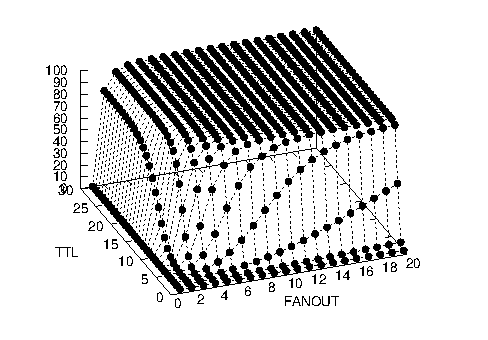
\includegraphics[width=\textwidth]{figs/hitratio.pdf}
	\caption{Caption...}
	\label{fig:related:2}
\end{figure}

% \Blindtext[1][1]

%\section{Conclusion}
%\label{sec:related:conclusion}
